\documentclass[a4paper,12pt]{scrartcl}
\usepackage[utf8]{inputenc}
\usepackage[UKenglish]{isodate}
\usepackage{csquotes}
\usepackage{graphicx}
\usepackage{wrapfig}
\usepackage{enumitem}
\usepackage{pdflscape}
\usepackage[toc,page]{appendix}
\usepackage{geometry}
\usepackage{hyperref}
\usepackage{cleveref}
\usepackage{listings}
\usepackage{csvsimple}
\usepackage{booktabs}
\usepackage{longtable}
\usepackage{caption}
\usepackage{subcaption}
\usepackage[colorinlistoftodos]{todonotes}
\usepackage[british]{babel}
\usepackage{float}
%\usepackage[margin=1in]{geometry}
\usepackage{listings}
\usepackage{color}
 
\definecolor{codegreen}{rgb}{0,0.6,0}
\definecolor{codegray}{rgb}{0.5,0.5,0.5}
\definecolor{codepurple}{rgb}{0.58,0,0.82}
\definecolor{backcolour}{rgb}{0.95,0.95,0.92}
 
\lstdefinestyle{mystyle}{
	language=PHP,
    backgroundcolor=\color{backcolour},   
    commentstyle=\color{codegray},
    keywordstyle=\color{magenta},
    numberstyle=\tiny\color{codegray},
    stringstyle=\color{codegreen},
    basicstyle=\footnotesize,
    breakatwhitespace=false,         
    breaklines=true,                 
    captionpos=b,                    
    keepspaces=true,                 
    numbers=left,                    
    numbersep=5pt,                  
    showspaces=false,                
    showstringspaces=false,
    showtabs=false,                  
    tabsize=3,
    morekeywords={ new, __halt_compiler, abstract, and, array, as, break, callable, case, catch, class, clone, const, continue, declare, default, die, do, echo, else, elseif, empty, enddeclare, endfor, endforeach, endif, endswitch, endwhile, eval, exit, extends, final, for, foreach, function, global, goto, if, implements, include, include_once, instanceof, insteadof, interface, isset, list, namespace, new, or, print, private, protected, public, require, require_once, return, static, switch, throw, trait, try, unset, use, var, while, xor}
}

\lstset{language=Java,
  showspaces=false,
  showtabs=false,
  breaklines=true,
  showstringspaces=false,
  breakatwhitespace=true,
  commentstyle=\color{pgreen},
  keywordstyle=\color{pblue},
  stringstyle=\color{pred},
  basicstyle=\ttfamily,
  moredelim=[il][\textcolor{pgrey}]{$$},
  moredelim=[is][\textcolor{pgrey}]{\%\%}{\%\%}
}
 
\lstset{style=mystyle}

\graphicspath{ {images/} }
\usepackage[
	backend=biber,
	style=ieee,
	]{biblatex}

\addbibresource{references.bib}

\title{829H1 Real Time Embedded Systems Exercise 1}
\author{Candidate No: 105936}
\date{\today}

\begin{document}
	
	\begin{titlepage}
		\maketitle
	\end{titlepage}
	
	\tableofcontents
	\newpage
	
	\section{Introduction}
	{
		
	}

	\section{Equipment}
	{
		\subsection{Hardware}{
			The experiments carried out in this report were run on the Freedom-K64F prototyping board\cite{nxpproducts2014}. To use this board we needed to connect the board to the computer using the debug port and copy across the program we wish to run and then press the reset button to load the program.
			\begin{figure}[h]
				\centering
				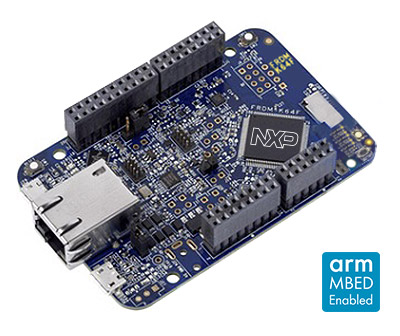
\includegraphics[width=0.5\textwidth]{FRDM-K64F-ANGLE}
				\caption{An Image of the Freedom-K64F Board used during experimentation\cite{nxpproducts2014}}
				\label{img:FRDM-K64F}
			\end{figure}
			Also in the last experiment we used and Oscilloscope to measure the voltage signals from the board to ensure that the program was working properly.
		}
		\subsection{Software}
		{
			To develop the experiments I used Arm's mbed cloud IDE. This allows users to write c++ code and compile it to a device of their choice. 
		}
	}
	
	\section{Experiments}
	{
		
	}

	\section{Conclusion}
	{
	
	}
	
	\newpage
	
	\printbibliography[heading=bibintoc,title=References]
\end{document}
